Man besitzt eine Eis-Firma, welche über den gesamten Verlauf des Jahres Eis produzieren soll. Da man jedoch keine Über- oder Unterproduktion, und damit Verluste, in Kauf nehmen möchte, versucht man mithilfe von Vorhersagen für das folgende Jahr seine Eisproduktion hieran anzupassen. Eine mögliche Vorhersage sieht folgendermaßen aus:

{{\centering
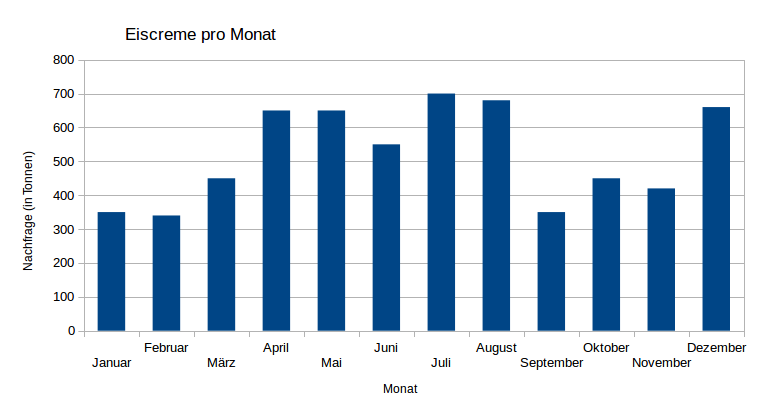
\includegraphics[width=\textwidth]{Grafiken/Eiscreme.png}}}

Bei der Erstellung des linearen Problems muss nun folgendes beachtet werden:
Die Änderung der Produktionsmenge von Monat A zu Monat B kostet 50€ pro Tonne.

Eis lässt sich lagern, jedoch kostet dies 20€ pro Tonne pro Monat.

Die Produktion von einer Tonne Eis kostet 1€

Es darf keine Unterproduktion vorliegen, d.h. der Bedarf muss gedeckt werden.

Zu Anfang des Jahres gibt es kein Eis, und zu Ende des Jahres darf ebenso kein Eis mehr vorhanden sein.

Dies liefert folgendes lineares Programm:
\begin{align*}
 \text{Minimiere:} &\sum_{m=1}^{12} (1 \cdot p_m + 50 \cdot (ci_m + cd_m) + 20 \cdot l_m) \\
 \text{Sodass für alle } m = 1, 2, \cdots ,12: \\
 p_m + l_m &\geq n_m  \\
 l_m &= p_{m-1} + l_{m-1} - n_{m-1} \\
 \sum_{m=1}^{12} p_m &= \sum_{m=1}^{12} n_m \\
 c_m &= p_{m} - p_{m-1} \\
 c_m &= ci_m - cd_m \\
 ci_m &\geq 0		\\
 cd_m &\geq 0
\end{align*}

Im folgenden wird nun diese Modellierung genauer erläutert:

\emph{Gleichung 1:} Für einen Monat $m$ in $M$, wobei $M = \{1, 2, \cdots, 12\}$ ist, muss die Produktionsmenge $p_m$, sowie die Menge der gelagerten Eiscreme $l_m$ größer als die Nachfrage $n_m$ sein.

\emph{Gleichung 2:} Die Menge des in einem Monat gelagerten Eis ist gleich der in vorherigen Monat übrig gebliebenen Menge Eis.

\emph{Gleichung 3:} Die insgesamt produzierte Menge an Eiscreme muss gleich der gesamten Nachfrage sein.

\emph{Gleichung 4:} Die Änderung der Produktionsmenge $c_m$ ergibt sich aus der Differenz der Produktionsmenge des Monates und des vorherigen Monates.
Man muss hierbei beachten dass sowohl negative als auch positive Änderungen kosten! Da man innerhalb eines linearen Problems jedoch nur mit linearen Funktionen arbeiten muss, müssen zwei Hilfsvariablen, $cd_m$ und $ci_m$ (decrease und increase) aufgestellt werden, welche mit Gleichungen 5, 6 und 7 definiert werden.
	
 Die absolute Gesamtänderung der Produktionsrate kann nun mit $ci_m + cd_m$ errechnet werden.

Zudem will man die Gesamtkosten minimieren, weshalb in einer optimalen Lösung $ci$ und $cd$ möglichst klein gewählt haben. Aus diesem Grund wird immer eine der Variablen $= 0$ sein.